% - - - -  - - - -  - - - -  - - - -  - - - -  - - - -  - - - -  - - - -  - - - -  - - - -  - - - -  - - - -  - - - -  - - - - 
\section{Introduction}

The classification of audio files and acoustic data is an ongoing area of research in Machine Learning. A recent article in \textit{Acoustics Today} outlined at least four areas where machine learning can augment traditional acoustics research \cite{AT}, and the annual Detection and Classification of Acoustic Scenes and Events (DCASE) challenge and workshop provides a forum for presenting research and techniques for sound analysis \cite{DCASE}. Applications of acoustic speech analysis include automatic speech recognition (ASR) systems and the development and optimization of voice assistants, like Siri or Alexa.

While ASR has come a long way, there is still room for improvement. For instance, Sheng \& Edmund report that ASR/voice assistants do not perform well for speakers with accents \cite{Sheng}. Having a model which could identify a speakers' accent could be the first step in improving the performance of ASR systems, which could lead to increased customer satisfaction.

The training of audio classifiers has been heavily influenced by advances in image classification \cite{Hershey}. Transfer learning has allowed well-trained image classifiers to be applied to audio data with fairly good success. For example, the VGGish audio classifier (see below) is based on the configuration of the VGG image classifier \cite{Hershey, VGG}. The current project seeks to employ transfer learning within the acoustic domain by using the VGGish model as the basis for classification of speech.  The goal is to see if a model trained for acoustic event detection can be leveraged to analyze speech data. Are the general acoustic features learned by the AED model sufficient to train a classifier for the narrower domain of human speech?
% - - - -  - - - -  - - - -  - - - -  - - - -  - - - -  - - - -  - - - -  - - - -  - - - -  - - - -  - - - -  - - - -  - - - - 
\section{VGGish}
As previously stated, this project uses the VGGish model as an acoustic feature extractor.  VGGish accepts as input audio files sampled at 16kHz, converts the files to mel spectrograms, and outputs an array of 128-dimensional features. In this project, the 128-dimensional features are then fed into a trainable classifier model. The pre-trained VGGish model is available on GitHub \url{https://github.com/tensorflow/models/tree/master/research/audioset/vggish} or through the Tensorflow Hub \url{https://tfhub.dev/google/vggish/1}.

\section{The Data}

The audio speech data came from the Speech Accent Archive, collected by \cite{AccentArchive} and available for download from Kaggle \url{https://www.kaggle.com/rtatman/speech-accent-archive}. The data includes demographic information about 2172 speakers, as well as 2138 audio recordings of speakers reading a fixed passage in English.  The demographic information records 9 features, including speaker ID, native language, birthplace, country, sex, and filename. The Speech Accent Archive also includes 2138 audio files, approximately one per speaker.

The text of the passage is: 
\begin{quotation}
Please call Stella.  Ask her to bring these things with her from the store:  Six spoons of fresh snow peas, five thick slabs of blue cheese, and maybe a snack for her brother Bob.  We also need a small plastic snake and a big toy frog for the kids.  She can scoop these things into three red bags, and we will go meet her Wednesday at the train station. \cite{AccentArchive}
\end{quotation}

\section{Data Wrangling}

The first step was to analyze the data for missing values. There were relatively few missing values in the metadata.  The four missing values in the birthplace column corresponded to synthesized audio files, so it made sense that the speaker would not have a birthplace. These records were also missing the value for "country". These files were dropped from the analysis, since the goal was to train a classifier on audio data from actual speakers. The one remaining missing value in the "country" column was for a speaker whose native language was Lao. The missing country value (Laos) was imputed from the other speakers with the same native language.

One of the columns in the metadata contained a boolean value to indicate whether the audio file for each speaker was missing or not. There were 32 records with missing audio files, and these records were dropped from the analysis, since they could not serve as input to the audio classifier models.

Upon trying to load the audio files from a list of speakers in the metadata, it was found that two additional speakers were missing audio files, so these speakers were dropped from the analysis.

Finally, there was one instance of speaker sex being recorded as 'famale', which was interpreted as a typo and changed to 'female'. 

% - - - -  - - - -  - - - -  - - - -  - - - -  - - - -  - - - -  - - - -  - - - -  - - - -  - - - -  - - - -  - - - -  - - - - 
\section{Exploratory Data Analysis}

After processing, the final dataset included roughly equal numbers of male and female speakers, as shown in Figure \ref{fig:GenderDistAll}.

\begin{figure}[h]
\begin{center}
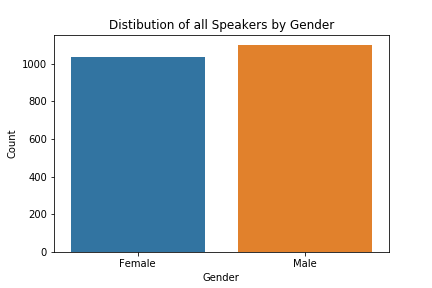
\includegraphics[width=4in]{GenderDistAll.png}
\caption{Distribution of Gender across all speakers.}
\label{fig:GenderDistAll}
\end{center}
\end{figure}

After processing, the data contained speakers from 199 native languages, 78 of which were represented by a single speakers.  English was the native language most represented, with 579 speakers. There are many different varieties of English spoken in the world. While we can't find out exactly which variety each speaker uses, we can infer the variety by looking at their birthplace and country. A majority of the native English speakers in the data are from the United States, followed by dozens of speakers from the UK, Canada and Australia, and fewer speakers from other countries and territories, as shown in Figure \ref{fig:EnglishCountry}.

\begin{figure}[h]
\begin{center}
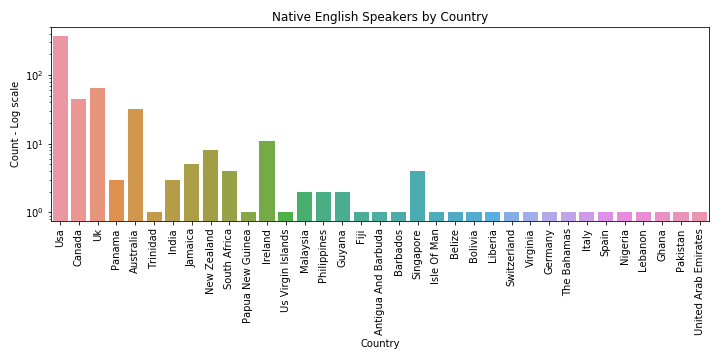
\includegraphics[width=6in]{EnglishCountry.png}
\caption{Distribution of native English speakers by country.}
\label{fig:EnglishCountry}
\end{center}
\end{figure}

After English, the ten most represented languages were selected for use in the Language Classifier. The number of speakers from these languages varied from 36 to 162, as shown in Figure \ref{fig:LangDistTop}.

\begin{figure}[h]
\begin{center}
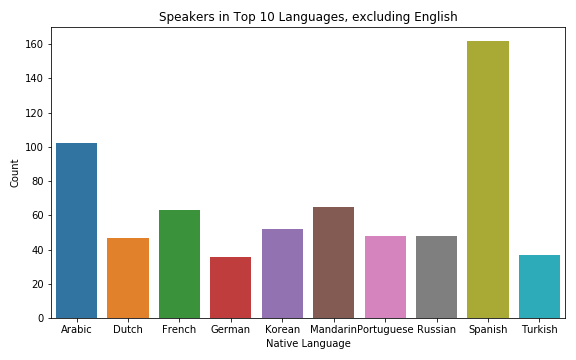
\includegraphics[width=4in]{TopLangCount.png}
\caption{Count of speakers in 10 languages with most speakers in dataset}
\label{fig:LangDistTop}
\end{center}
\end{figure}

% - - - -  - - - -  - - - -  - - - -  - - - -  - - - -  - - - -  - - - -  - - - -  - - - -  - - - -  - - - -  - - - -  - - - - 
\section{Audio File Processing}

The VGGish model accepts audio files as input and output arrays of feature embeddings. The original VGGish model was trained on 10 second audio files. Before being fed to the VGGish model, the audio files from the database were normalized, divided into 10s segments, and augmented with random noise.

Given the length of the reading passage, the audio files for most speakers were longer than 20s. Dividing the files into 10s segments accomplished several things. First, it supplied audio files for the VGGish models that were the same length as the VGGish training files. Second, it insured that the dimensions of the VGGish output would be consistent, since all of the input files would be of the same length. Finally, it increased the number and variability of files available for the training and testing of the new classifier models, which should lead to more robust models.

\begin{figure}[h]
\begin{center}
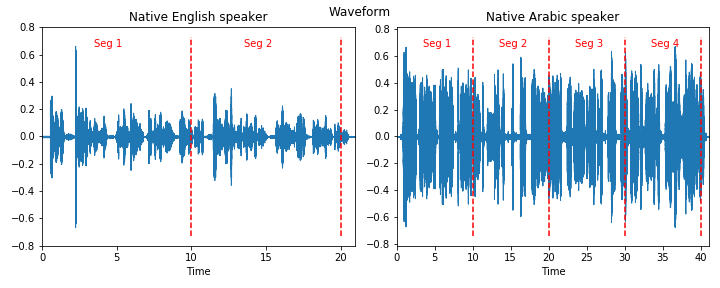
\includegraphics[width=5in]{Waveforms.png}
\caption{Waveforms of audio for speakers English11 and Arabic24. Dashed red lines show 10s segments that will be saved upon segmentation. }
\label{fig:Waveform}
\end{center}
\end{figure}

Since the original audio files differed in length between speakers, the number of segments per speakers was not consistent. As shown in Figure \ref{fig:Waveform}, the audio file from a native English speaker was just over 20 seconds long, as was divided into two segments. The file from a native Arabic speaker, by contrast, was over 40 seconds long, and was divided into four segments. Each segment was saved as a separate .wav file.

Once the original audio files had been segmented and saved, the segments were augmented by adding randomly generated, low-level 'noise', as shown in Figure \ref{fig:Noise}. The addition of noise should improve models robustness, since the model will learn to focus on salient acoustic features, while ignoring the noise. The noisy segments and the original segments were saved in separate files, thus doubling the number of files available for model training.

\begin{figure}[h]
\begin{center}
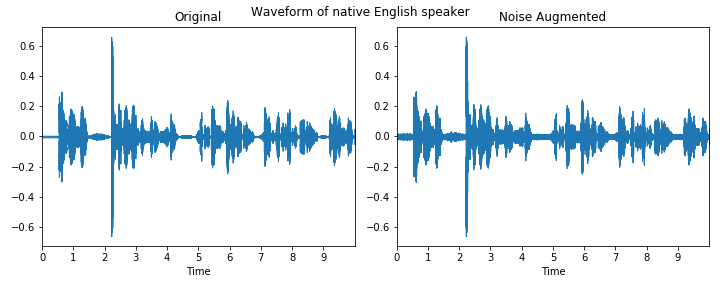
\includegraphics[width=5in]{OrigNoise.png}
\caption{Waveforms of original (left) and noise augmented (right) segments from speaker English11. The low-level, random noise is most noticeable when comparing portions where the original waveform has little sound (e.g. 0-0.25 s, 4.25-4.75 s).}
\label{fig:Noise}
\end{center}
\end{figure}

Internally, the VGGish model converts the audio files to a Mel spectrogram, which is then run through the convolutional layers to produce the feature embedding. An example of a Mel spectrogram is provided in the right panel of Figure \ref{fig:MelSpec}.

\begin{figure}[h]
\begin{center}
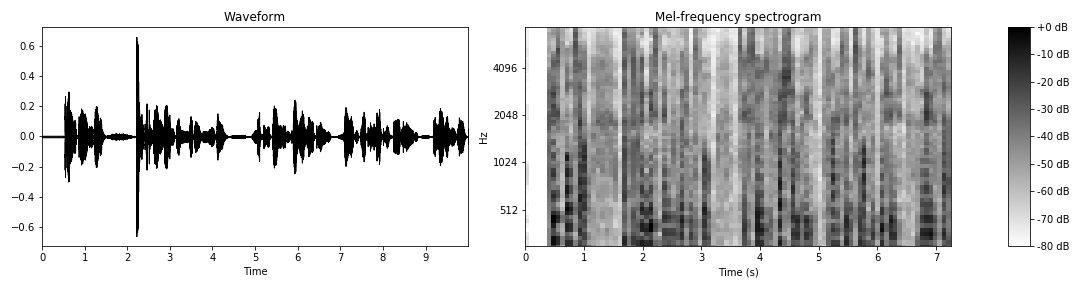
\includegraphics[width=5in]{English11MelSpec.png}
\caption{Waveform (left) and Mel spectrogram (right) of a segment from speaker English11. The VGGish model converts audio input files to a Mel spectrogram, which is then fed through its convolutional layers.}
\label{fig:MelSpec}
\end{center}
\end{figure}

Two different classifier categories were built as part of this project - one to predict the gender of the speaker, and one to predict the native language of the speaker. While the audio processing steps outlined above applied to the input for both classifiers, the training and testing data, and the structure of the models varied between the classifiers, so they will be addressed separately below.
% - - - -  - - - -  - - - -  - - - -  - - - -  - - - -  - - - -  - - - -  - - - -  - - - -  - - - -  - - - -  - - - -  - - - - 
\section{Gender Classifier}
\subsection{Data Subsets}

The goal of the Gender Classifier is to predict speaker gender (female and male, coded as 0 and 1, respectively) from the audio input. All of the speakers from the Speech Accent Archive were used for the Gender Classifier. First, the speakers were split into training, validation and testing sets.  Next, the audio files for each dataset were segmented. Then, the segments in the training and validation datasets were augmented with noise. Since there was not a  consistent number of segments per speaker, and since the testing file were not augmented with noise, the distribution of speakers and segments in the training and testing sets differed, as shown in Figure \ref{fig:GenderDist}. Most notably, while there were fewer speakers in the validation set than the testing set, once the files were segmented and augmented, there were more segments in the validation set. However, the distribution of male and female speakers/segments remained fairly consistent among the datasets.

\begin{figure}[h]
\begin{center}
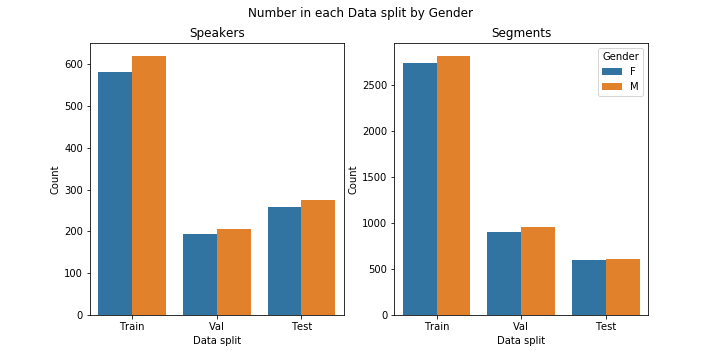
\includegraphics[width=4in]{Gen_NSegSpeakSplit.png}
\caption{Number of speakers (left) and segments (right) by gender in each data split for the Gender Classifier.}
\label{fig:GenderDist}
\end{center}
\end{figure}

\subsection{Model Architecture}
Two different models were trained and evaluated for the gender classifier. The structure of each model is shown in Table \ref{tab:GenModels}. 

The models had identical input and output layers. The shape of the input was (32, 10, 128), which corresponds to the batch size (32) and the VGGish embedding (10, 128).  Since the classification was binary, the output layer contained one node, with a sigmoid activation function.

The models differ in the number of hidden layers. Each hidden layer consisted of a dense layer followed by a dropout layer with a dropout rate of 50\%. The first model contained a single hidden layer with 128 nodes. The second model contained two hidden layers, the first with 128 nodes, and the second with 64 nodes. Prior to being fed into the output layer, the output from the previous layer was flattened into a 1D array. The shape of the flattened array varied for each model, based on the number of nodes of the prior layer (128 vs 64).

\begin{table}[!h]
\begin{center}
\caption{Structure of the two gender classifier models. Model 1 has one hidden layer with 128 nodes, while Model 2 has two hidden layers with 128 and 64 nodes, respectively.}
\begin{tabular}{l | c | c |}

Layer  & Model 1 & Model 2\\
\hline

Input 	& (32, 10, 128) & (32, 10, 128) \\ \hline

Dense	& 128 nodes & 128 nodes \\
Dropout	& 50\%		& 50 \% \\ \hline

Dense	&			& 64 nodes \\
Dropout	& 			& 50\% \\ \hline

Flatten 	& (32, 1280)	& (32, 640) \\ \hline
Output 	& (32, 1)		& (32, 1)\\
\hline
\end{tabular}
\label{tab:GenModels}
\end{center}
\end{table}

% - - - -  - - - -  - - - -  - - - -  - - - -  - - - -  - - - -  - - - -  - - - -  - - - -  - - - -  - - - -  - - - -  - - - - 
\subsection{Model Performance and Evaluation}

Each model was set to run for 100 epochs, or until the validation loss stopped decreasing for 5 consecutive epochs. Model 1 trained for 8 epochs, with the lowest validation loss found at epoch 3. Model 2 trained for 7 epochs, with the lowest validation loss at epoch 2. The evaluation metrics below are based on the weights of the models with the lowest validation loss - after epochs 3 and 2, respectively.

As shown in Table \ref{tab:GenMetricsSum} and Table \ref{tab:GenConfusion}, both models performed quite well on the binary classification task, reaching an accuracy of 98.14\% and 97.55\%, respectively. Model 1 showed similar performance between both classes, with nearly equal numbers of speakers being misclassified from each class. Model 2 showed more discrepancies between the performance of the two classes. Male voices were identified correctly at a rate of 99.14\%, while female voices were identified correctly only 96.5\%. However, the precision of the predictions was the reverse - the precision of female voice prediction was 99.14\%, while the precision of male voice prediction was 96.02\%.

\begin{table}[h]
\begin{center}
\caption{Gender Classifiers - Metrics Comparison}
\begin{tabular}{l c c}
& 	Model 1 & Model 2 \\ \hline
Loss	&0.061640 & 0.076962 \\
Accuracy& 0.981419 & 0.975507 \\
Precision & 0.982818 & 0.960199 \\
Recall & 0.979452 & 0.991438 \\
\end{tabular}
\label{tab:GenMetricsSum}
\end{center}
\end{table}

Model 1, with similar performance between genders, is a good model for general use, where a balance between either sensitivity and specificity, or precision and recall is desired. Model 2 would be preferred in cases where optimizing specificity/recall is desired, in other words, if there is high cost for misclassifying a male voice, but lower cost for misclassifying a female voice.

\begin{table}[h]
\begin{center}
\caption{Confusion Matrices for the Gender Classifier Models}
\begin{tabular}{l l | c c r }
\multicolumn{2}{l}{\textbf{Model 1}} & \multicolumn{2}{c}{Predicted} & Recall \\
& & F & M &  \\ 
\cline{2-5}
Actual & F & 590 &  10 & 0.9833 \\
& M & 12 & 572 & 0.9795 \\  \hline
Precision&  & 0.9801 & 0.9828 \\ 
Accuracy & & &  & 0.9814 \\
\end{tabular}
\begin{tabular}{l l | c c r }
\multicolumn{2}{l}{\textbf{Model 2}} & \multicolumn{2}{c}{Predicted} & Recall \\
& & F& M &  \\ 
\cline{2-5}
Actual & F & 576 &  24 & 0.9650 \\
& M & 5 & 579 & 0.9914 \\  \hline
Precision&  & 0.9914 & 0.9602 \\ 
Accuracy & & &  & 0.9755 \\
\end{tabular}
\label{tab:GenConfusion}
\end{center}
\end{table} 

%Could add:
% Add research about Classifier models - Are male vs female voices harder to classify? Why would we want different rates of precision or recall for the different genders?


% - - - -  - - - -  - - - -  - - - -  - - - -  - - - -  - - - -  - - - -  - - - -  - - - -  - - - -  - - - -  - - - -  - - - - 
\section{Language Classifier}

The goal of the Language Classifier was to identify the native language of the speaker, given that all speakers read the same passage in English. To limit the scope of the classifier, the ten most represented languages in addition to English were selected for use in the Language Classifier, as shown above in Figure \ref{fig:LangDistTop}. The labels for the classifier were one-hot encoded into a 1x11 array.

\subsection{Data Subsets}
The selected data contained many more speakers of English, Spanish and Arabic than speakers of other languages. To balance the classes for the Language Classifier, the number of speakers for these three languages was downsampled to 75, which meant that each of these language classes contained 12.0773\% of the total number of speakers in the dataset. German had the fewest number of speakers (36), which comprised 5.797\% of the speakers. The distribution of the number of speakers sampled per language class is shown in blue in Figure \ref{fig:LangDistTot}. The speakers of each language were split separately into training, validation, and testing sets, so the distribution of speakers per language in each data split reflects the overall distribution of speakers.

\begin{figure}[h]
\begin{center}
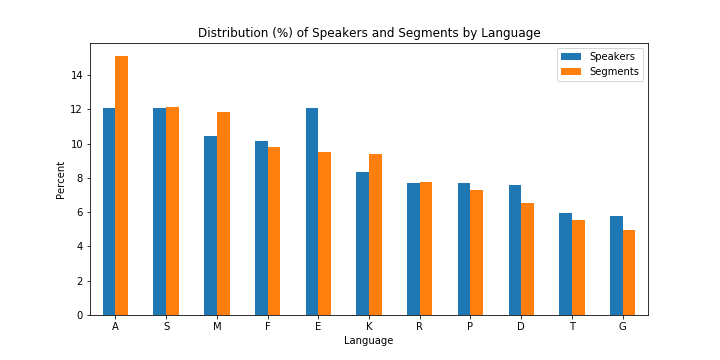
\includegraphics[width=5in]{LangDistPercentSpSeg.png}
\caption{Distribution of Speakers and Segments by Language}
\label{fig:LangDistTot}
\end{center}
\end{figure}

After the speakers were splits into training, validation and testing sets, the audio files for all speakers were segmented, and the segments in the training and validation splits were augmented with noise. Since the number of segments per speaker was dependent on the length of the original audio file, which was not determined before the speakers were split, the number of segments per language and per data split were not identical to the distribution of the speakers. Like with the Gender Classifier data, the validation data contained fewer speakers, but more segments than the test data.

While the distribution of speakers and segments for most of the languages remains similar (seen by comparing the heights of the blue and orange bars in Figure \ref{fig:LangDistTot}), the distribution of Arabic and English segments changed dramatically. While there were equal numbers of Arabic and English speakers, there were 380 Arabic segments compared to 239 English segments. Thus, the distribution of Arabic segments grew to 15.109344\% of the segments, while English segments shrank to 9.502982\%, moving English behind Spanish, Mandarin and French.

% - - - -  - - - -  - - - -  - - - -  - - - -  - - - -  - - - -  - - - -  - - - -  - - - -  - - - -  - - - -  - - - -  - - - - 
\subsection{Model Architecture}

Three models were trained and evaluated for the language classifier. The structure of each model is shown in Table \ref{tab:LangModels}. 

All of the models had identical input and output layers. The shape of the input was (32, 10, 128), which corresponds to the batch size (32) and the VGGish embedding (10, 128).  There were 11 possible classes, so the output layer consisted of 11 nodes. A softmax activation function was used on the output layer, so that the output vector contained the probability that the speaker belonged to each of the output classes. The class with the highest probability was taken to the be predicted class.

The models differ in the number of nodes and the number of hidden layers. Each hidden layer consisted of a dense layer followed by a dropout layer with a dropout rate of 50\%. The first model contained a single hidden layer with 12 nodes, while the second model had a single layer with 128 nodes. The third model contained two hidden layers, the first with 128 nodes, and the second with 64 nodes. Prior to being fed into the output layer, the output from the previous layer was flattened into a 1D array. The shape of the flattened array varied for each model, based on the number of nodes of the prior layer (12 vs 128 vs 64).

\begin{table}[!h]
\begin{center}
\caption{Language Classifier Model Architectures. Model 1 has one hidden layer with 12 nodes, Model 2 has one hidden layer with 128 nodes, and Model 3 has two hidden layers with 128 and 64 nodes, respectively.}
\begin{tabular}{l | c |c  | c |}

Layer  & Model 1 & Model 2 & Model 3\\
\hline

Input 	& (32, 10, 128)& (32, 10, 128) & (32, 10, 128) \\ \hline

Dense	& 12 nodes 	& 128 nodes 	& 128 nodes \\
Dropout	& 50\%		& 50\%		& 50 \% \\ \hline

Dense	&			&			& 64 nodes \\
Dropout	&			& 			& 50\% \\ \hline

Flatten 	& (32, 120)	& (32, 1280)	& (32, 640) \\ \hline
Output 	& (32, 11)		& (32, 11)		& (32, 11)\\
\hline
\end{tabular}

\label{tab:LangModels}
\end{center}
\end{table}

% - - - -  - - - -  - - - -  - - - -  - - - -  - - - -  - - - -  - - - -  - - - -  - - - -  - - - -  - - - -  - - - -  - - - - 
\subsection{Model Performance and Evaluation}

Each model was set to run for 100 epochs, or until the validation loss stopped decreasing for 5 consecutive epochs. Model 1 trained for 19 epochs with lowest validation loss at epoch 15, Model 2 trained for 8 epochs, with the lowest validation loss at epoch 3, and Model 3 trained for 11 epochs with the lowest validation loss at epoch 6.The metrics below are based on the final trained models, with weights from the last trained epoch.

A naive classifier that always predicted the majority class (Arabic) would have an accuracy of 15\%.  All three of the models improved upon this baseline accuracy rate, as shown in the second row of Table \ref{tab:LangMetricsSum}. While Model 1 has the highest precision rate, it has the lowest accuracy, recall and F1 scores, and will not be considered further. Model 2 has the highest recall and F1 scores, but also the lowest precision. The most complicated model, Model 3, has the highest overall accuracy, and has F1 scores only slightly lower than Model 2. 

The main difference between Models 2 and 3 s in their precision - Model 2 has precision of only 50\%, while the precision of Model 3 is 60.5\%. One difference between the models that can explain this discrepancy is the frequency with which the model predicts each language classes. Model 2 distributes the predictions more equally between all of the language classes, while Model 3 had several classes with few predictions, and several with many predictions. A comparison of the number of predictions per class generated by these two models is given in Table \ref{tab:LangPredict}.  Another difference between the Model 2 and Model 3 is the number of classes for which no correct predictions are made: Model 2 only makes no correct predictions for German, while Model 3 makes no correct prediction for German, Russian, and Portuguese.

\begin{table}[h]
\begin{center}
\caption{Language Classifiers - Metrics summary}
\begin{tabular}{l c c c}
		&Model 1		&Model 2		&Model 3 \\ \hline
Loss		&2.25485		&2.323		&2.20684 \\
Accuracy	&0.232955	&0.238636	&0.25\\
Precision	&0.625		&0.5			&0.605263\\
Recall	&0.0142045	&0.0738636	&0.0653 \\ 

F1 Macro	&0.16999		&0.195512	&0.191103\\
F1 Weighted	&0.20067	&0.228178	&0.224565\\
\end{tabular}
\label{tab:LangMetricsSum} 
\end{center}
\end{table} 

\begin{table}[h]
\begin{center}
\caption{Language Classifiers - Predictions per Class}
\begin{tabular}{l c  c}
	& Model 2	& Model 3 \\ \hline
Mean	&32		& 32\\
Minimum	&14		& 2\\
Median	&23		& 38 \\
Maximum	&68		& 63	\\
SD		&17.09	&22.36\\ 

\end{tabular}
\label{tab:LangPredict} 
\end{center}
\end{table} 

Given the slightly higher rate of precision and accuracy, Model 3 has been chosen as the final model. A confusion matrix of the prediction generated by this model are shown in Table \ref{tab:LangConfMat}, with the recall, precision and F1 score for each class in Table \ref{tab:LangClassReport}.

Not surprisingly, the class with the highest number of correct predictions was the majority class, Arabic, with 24/55 segments correctly predicted (recall of 0.43.63\%) and 24/52 predictions being correct (precision of 0.46.15\%). Dutch, Spanish, English, and Mandarin had 12-15 correct predictions per class. German, the smallest class, along with Russian and Portuguese, had no correct predictions, while Turkish has a single correct prediction.

Behind Arabic, Spanish and Mandarin contributed about the same number of segments to each of the training sets (12.167\% and11.84 \%, respectively). Interestingly, the model made 63 predictions for Spanish and 62 predictions  for Mandarin, which is more than it predicted the majority class. However, since there were fewer correct predictions for Mandarin (15) and Spanish (12), the precision rates for these classes is roughly half that of Arabic.

While Dutch contributed only 6.520875\% of the segments overall, almost half of its testing files were correctly predicted (12/25), making it the class with the highest recall (48\%).

\begin{table}
\begin{center}
\caption{Confusion matrix for Model 3 predictions. The bold numbers on the diagonal represent correct predictions.}
\begin{tabular}{l | c c c c c c c c c c c || c}
Lang			&R &A &T &K &G &D &S &F &E &P &M & Segments\\ \hline
Russian		&\textbf{0}  &2  &1  &4  &0  &1  &7  &4  &1  &1  &7 &28\\
Arabic		&0 &\textbf{24}  &0  &4  &1  &7  &2  &2  &4  &0 &11 &55\\
Turkish		&0  &1  &\textbf{1}  &4  &0  &3  &4  &0   &2  &1  &5 &21\\
Korean		&1 &10  &0  &\textbf{6}  &0  &3  &2  &2  &4  &2  &1 &31\\
German		&0  &0  &0  &1  &\textbf{0}  &0  &5  &1  &5  &2  &1 &15\\
Dutch		&0  &4  &0  &0  &0 &\textbf{12} & 3  &1  &3  &1  &1 &25\\
Spanish		&1  &2  &0  &6  &2  &1 &\textbf{12}  &3  &8  &0  &7 &42\\
French		&1  &3  &0  &4  &1  &2 &10 & \textbf{5}  &1  &1  &4 &32\\
English		&0  &1  &0  &3  &0  &5  &2  & 2 &\textbf{13}  &0  &4 &30\\
Portuguese	&0  &3  &0  &3  &1  &0  &7  & 5  & 3  &\textbf{0}  &6 &28\\
Mandarin		&0  &2 & 0  &8  &2  &4  &9  & 1  & 2  &2 &\textbf{15} &45\\ \hline
Total Predictions&3 &52 &2 &43 &7 &38 &63 &26 &46 &10 &62 &\textbf{352}\\

\end{tabular}
\label{tab:LangConfMat}
\end{center}
\end{table}

% - - - -  - - - -  - - - -  - - - -  - - - -  - - - -  - - - -  - - - -  - - - -  - - - -  - - - -  - - - -  - - - -  - - - - 
\begin{table}
\begin{center}
\caption{Model 3 Metrics by Language}
\begin{tabular}{l c c c| c}
Language  &Precision &Recall &F1-score&Samples\\ \hline
Russian	&0.00	&0.00	&0.00	&28\\
Arabic	&0.46	&0.44	&0.45	&55\\     
Turkish	&0.50	&0.05	&0.09	&21\\      
Korean	&0.14	&0.19 	&0.16	&31\\      
German	&0.00	&0.00	& 0.00 	&15\\       
Dutch	&0.32	&0.48	&0.38	&25\\   
Spanish	&0.19	&0.29	&0.23	&42\\      
French	&0.19	&0.16	&0.17	&32\\    
English	&0.28	&0.43	&0.34	&30\\  
Portuguese&0.00	&0.00	&0.00	&28\\    
Mandarin	&0.24	&0.33	&0.28	&45\\ \hline
      
accuracy		&		&		&0.25	&352\\
macro avg		& 0.21	&0.22	&0.19	&352\\
weighted avg	& 0.23	&0.25	&0.22	&352\\ \hline
\end{tabular}
\label{tab:LangClassReport}
\end{center}
\end{table}

% - - - -  - - - -  - - - -  - - - -  - - - -  - - - -  - - - -  - - - -  - - - -  - - - -  - - - -  - - - -  - - - -  - - - -
\subsection{Discussion}
One question about the language classifier was whether it would identify similarities between languages with historical similarities. For example, Spanish, French and Portuguese are all descendants of Latin, and are more closely related to each other than to other languages in this database, so it would not be surprising for them to be confused with each other more often than with other, unrelated languages.  However, the language classifier showed only weak connections between some related languages. It appears that the weight of a language class in the data may play a larger role that similarities between related languages.

For example, Portuguese segments were misclassified as French 5 times and Spanish 7 times, but were identified as Mandarin 6 times, and misclassified as Arabic, Korean and English 3 times each. Arabic, Spanish, Mandarin, and French, in that order, are the top languages in the data. The presence of so many Mandarin misclassifications suggests that the classification of the Portuguese samples was based on class weights more than on language relatedness.

Likewise, French segments were misclassified as Spanish 10 times, but were more likely to be classified as Korean and Mandarin (4 times each) than Portuguese(1), which was fourth from the bottom in terms of class weight. Spanish samples were only misclassified as French 3 times, but as Mandarin 7 times and Korean 6 times, even though Mandarin and Korean are not related to Spanish. Of the samples that were misclassified as Spanish, 10 were actually French and 7 were Portuguese, but 9 were Mandarin and 7 were Russian. So, while there are weak patterns of misclassification between the Romance languages, Mandarin and Korean also show similar levels of misclassification with Spanish, French and Portuguese. 

Another trio of closely-related languages - English, Dutch and German - showed even weaker patterns of misclassification, with Dutch and German never being confused for one another, and only 3 Dutch segments and 5 German segments misclassified as English, and 5 English segments misclassified as Dutch. Since there were relatively few segments of Dutch (4.97\%) and German (6.52\%) in the data, it may not be surprising that they were not often predicted.

\subsection{Future directions}
There are several ways that future Language Classifier models could be optimized further. From a model architecture standpoint, more models could be developed that included more layers and/or more nodes, had different dropout proportions, or used different activation functions.  From a phonetic/acoustic standpoint, there may be additional acoustic features, like tempo/beat tracking, or the duration of the original file, that could be added to improve discrimination between phonetically different accents. Another possible feature to include in the model could be an accentedness rating - how native-like or non-native-like the speech sounds to a native speaker. While this rating would not necessarily be available for future samples (in production), it could be useful for training.

While imbalanced data is prevalent in the real world, it is possible that using a more balanced data set, either by downsampling the existing data, or by collecting more speech samples from underrepresented languages, would increase model performance. Finally, a model trained to distinguish between fewer languages would have better accuracy, if the final use case involved processing audio files from only a subset of the language classes.
% - - - -  - - - -  - - - -  - - - -  - - - -  - - - -  - - - -  - - - -  - - - -  - - - -  - - - -  - - - -  - - - -  - - - - 
\section{Conclusion}
The goal of this project was to use a model pre-trained for acoustic event detection and evaluate if the extracted features were useful for analyzing speech. In both cases, the features extracted by the VGGish model were useful for training classifiers to classify speaker characteristics from audio files. The VGGish embeddings were sufficient to train a Gender Classifier with 98\% accuracy. The Language Classifier based on the VGGish features showed improvement over a model that only predicted the majority class. Transfer learning has been shown to be useful for training new models, even with slightly different domains, with smaller datasets in relatively short amounts of time.